\documentclass{article}

\usepackage{booktabs}
\usepackage{tabularx}
\usepackage{hyperref}
\usepackage{graphicx}
\usepackage{float}
\usepackage{array}
\usepackage{pdflscape}
\usepackage{longtable}

\hypersetup{
    colorlinks=true,       % false: boxed links; true: colored links
    linkcolor=red,          % color of internal links (change box color with linkbordercolor)
    citecolor=green,        % color of links to bibliography
    filecolor=magenta,      % color of file links
    urlcolor=cyan           % color of external links
}

\title{Hazard Analysis\\\progname}

\author{\authname}

\date{}

\input{../Comments}
%% Common Parts

\newcommand{\progname}{Software Engineering} % PUT YOUR PROGRAM NAME HERE
\newcommand{\authname}{Team \#2, Team Name
\\ Zihao Du 
\\ Matthew Miller
\\ Firas Elayan
\\ Abhiram Neelamraju
\\ Michael Kim} % AUTHOR NAMES                  

\usepackage{hyperref}
    \hypersetup{colorlinks=true, linkcolor=blue, citecolor=blue, filecolor=blue,
                urlcolor=blue, unicode=false}
    \urlstyle{same}
                                


\begin{document}

\maketitle
\thispagestyle{empty}

~\newpage

\pagenumbering{roman}

\begin{table}[hp]
\caption{Revision History} \label{TblRevisionHistory}
\begin{tabularx}{\textwidth}{llX}
\toprule
\textbf{Date} & \textbf{Developer(s)} & \textbf{Change}\\
\midrule
Oct 20th & All & Revision 0\\
... & ... & ...\\
\bottomrule
\end{tabularx}
\end{table}

~\newpage

\tableofcontents

~\newpage

\pagenumbering{arabic}

\section{Introduction}

Based on the STPA Handbook, a system hazard is a system state or set of conditions that, together with a particular set of worst-case environmental conditions will lead to a loss. Regarding CampusConnections, our AR-based social networking application, a hazard can be a condition in the game when it fails to perform the intended functions or performs unexpected behaviors when coupled with environmental conditions. This document aims to detect, analyze, assess, and eliminate or migrate potential safety and security hazards that are applicable to this application. 

\section{Scope and Purpose of Hazard Analysis}

The scope of hazard analysis is to specify all potential system hazards that may arise when using the application and discover safety and security requirements to migrate and eliminate the effects of those hazards. However, it will not include hazards related to the hardware the application is running on. It will be the choice of the user and we cannot account for all mobile devices on the market. Hazard to the user and the society will be out of the scope as well. We will assume users intend to run the application on a normally functioning mobile device properly and efficiently. The purpose of the document is to highlight various hazards associated with the system, effects and causes of corresponding failures along with new requirements for further mitigation steps.

\section{System Boundaries and Components}
The system will be divided into the following components:
\begin{enumerate}
	\item The application's in-game feature components:
	      \begin{itemize}
		      \item Social Media
		      \item AR \& Location Services
		      \item Event/Lecture Management
		      \item General application features
	      \end{itemize}
	\item The database being used which will store all of users' data
	
\quad General app features include user login system, it will be responsible for user login and account creation, as well as notification and user accessibility management. The other three features are just responsible for corresponding in-game functionalities, more details can be found in the figure below. The database and user interaction are considered external to the system, the interaction between the system and external systems is described in the previous \href{https://github.com/beatlepie/4G06CapstoneProjectTeam2/blob/docs-hazard-analysis/docs/SRS-Volere/SRS.pdf}{document}.
\end{enumerate}
\begin{figure}[H]
\begin{center}
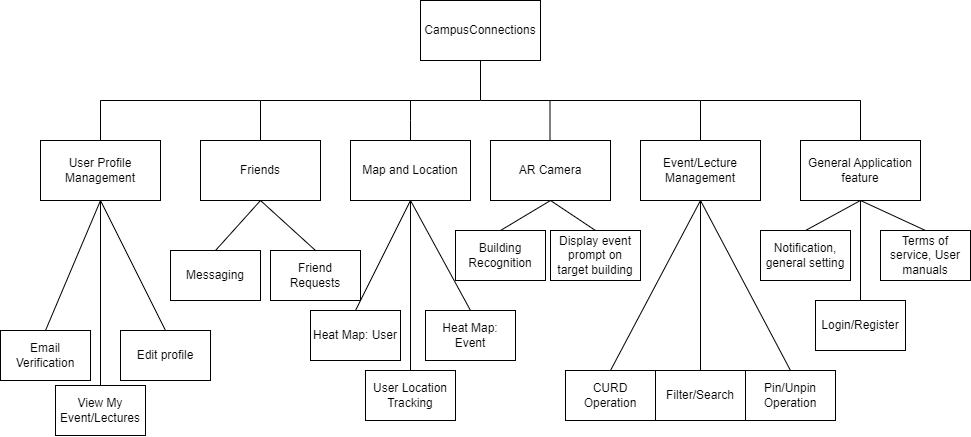
\includegraphics[scale=0.7]{components.png}
\end{center}
\caption{System Components}
\end{figure}
\section{Critical Assumptions}

\begin{itemize}
    \item Assume the users of the application do not intend to misuse it
    \item Assume the user's device will have all necessary hardware components with sufficient computing/output power such as sensors, processors, etc.
    \item Assume the routes to the backend of the system will always be ready to serve requests and not blocked due to unnecessarily locked resources
\end{itemize}

\section{Failure Mode and Effect Analysis}

\wss{Include your FMEA table here}

\begin{landscape}
    \begin{longtable}{|>{\hspace{0pt}}m{0.075\linewidth}|>{\hspace{0pt}}m{0.102\linewidth}|>{\hspace{0pt}}m{0.106\linewidth}|>{\hspace{0pt}}m{0.156\linewidth}|>{\hspace{0pt}}m{0.169\linewidth}|>{\hspace{0pt}}m{0.242\linewidth}|>{\hspace{0pt}}m{0.033\linewidth}|>{\hspace{0pt}}m{0.044\linewidth}|} 
    \hline
    \multicolumn{1}{|>{\centering\hspace{0pt}}m{0.075\linewidth}|}{Design Function} & \multicolumn{1}{>{\centering\hspace{0pt}}m{0.102\linewidth}|}{Failure Modes} & \multicolumn{1}{>{\centering\hspace{0pt}}m{0.106\linewidth}|}{Causes of Failure}                                 & \multicolumn{1}{>{\centering\hspace{0pt}}m{0.156\linewidth}|}{Effects of Failure}                                    & \multicolumn{1}{>{\centering\hspace{0pt}}m{0.169\linewidth}|}{Detection}                & \multicolumn{1}{>{\centering\hspace{0pt}}m{0.242\linewidth}|}{Recommended Action}                                                     & \multicolumn{1}{>{\centering\hspace{0pt}}m{0.033\linewidth}|}{SR} & \multicolumn{1}{>{\centering\arraybackslash\hspace{0pt}}m{0.044\linewidth}|}{Ref. No.}  \endfirsthead 
    \hline
    F21: AR Object Recognition                                                      & App is unable to detect object                                               & - Poor lighting conditions\par{} - Camera angle                                                                  & User is unable to view information from the AR element                                                               & Keep track of prior incomplete scan attempts                                            & Implement a failsafe mechanism that shows the scannable information if enough previous attempts have failed                           &                                                                   &                                                                                         \\ 
    \hline
    14.1 Backend Server                                                             & Server is inaccessible                                                       & - No internet connection\par{} - Hosting service is down\par{} - Invalid access key                              & - Users are unable to make changes to their profile\par{} - Users cannot receive updated information from the server & Keep track of the connection to the server using periodic heartbeats or similar methods & Display an error message stating that the connection the the server has been lost                                                     &                                                                   &                                                                                         \\ 
    \hline
    User Profile View                                                               & Sensitive user data is publicly visible                                      & - Invalid visibility permissions\par{} - Access control software malfunction                                     & Confidential user information could be exposed and used for malicious purposes                                       & Software failsafes and checks that verify the integrity of the permission structure     & Prevent other users from accessing unauthorized information by creating a robust permissions system                                   &                                                                   &                                                                                         \\ 
    \hline
    12 App Performance                                                              & App performance is poor                                                      & - Large amounts of assets to be rendered\par{} - Slow internet connection\par{} - App is running on an old phone & - User experiences lag or slowdown\par{} - App feels unresponsive                                                    & Track of frame times or other performance metrics                                       & Only show up to a maximum number of avatars or lower the level of detail                                                              &                                                                   &                                                                                         \\ 
    \hline
    12.2 User Safety                                                                & App is used where and when it is not intended                                & - User is distracted by the app                                                                                  & - User could get into an accident                                                                                    & N/A                                                                                     & Display a warning message when opening the app that tells the user to be aware of their surroundings at all times while using the app &                                                                   &                                                                                         \\ 
    \hline
    AR Module                                                                       & Device is not compatible with AR features                                    & Device is missing required hardware or software                                                                  & User cannot use the AR features                                                                                      & Check if device supports the required feature set using API functions.                  & Display a warning message if the user's device is not compatible                                                                      &                                                                   &                                                                                         \\
    \hline
    \end{longtable}
    \end{landscape}

\section{Safety and Security Requirements}

\wss{Newly discovered requirements.  These should also be added to the SRS.  (A
rationale design process how and why to fake it.)}

\subsection{Safety Requirements}
\begin{itemize}
    \item The product shall not transmit information while not in use.
    \begin{itemize}
        \item \textbf{Rationale:} This requirement limits the battery usage of the product.
        \item \textbf{Fit Criterion:} The product will not execute any code that involves the transmission of information outside of the product.
    \end{itemize}
\end{itemize}

\subsection{Access Requirements}

\subsection{Integrity Requirements}

\subsection{Privacy Requirements}

\subsection{Audit Requirements}

\subsection{Immunity Requirements}

\section{Roadmap}

\wss{Which safety requirements will be implemented as part of the capstone timeline?
Which requirements will be implemented in the future?}

Safety Requirements to be implemented for capstone:
\begin{itemize}
    \item The product shall not transmit information while not in use.
\end{itemize}

Safety Requirements to be implemented after capstone:
\begin{itemize}
    \item
\end{itemize}
\end{document}